% Chapter 1

\chapter{Neural Networks Architectures} % Main chapter title

\label{nnarch} % For referencing the chapter elsewhere, use \ref{Chapter3} 

\lhead{Chapter 3. \emph{Neural Networks Architectures}} % This is for the header on each page - perhaps a shortened title

%----------------------------------------------------------------------------------------
This chapter will explore the ways to construct a Neural Network. We will develop some basic elements (i.e. Neurons and Layers) that can combined in several ways, much like a child's toy building bricks to design large netowkrs capable of representing complex functions. We will also present the various ways of interpreting the working of a such networks and seek to apply these empirically developed intuitive rules to provide general guidelines while using the networks in practice.\\

An important result of the late 20th century was the proof by Hornik et al., that a feedforward network with a linear output layer containing at least one hidden layer, and any activation function, which non-linearly constrains the output of each neuron to lie in a finite range (such as
the logistic sigmoid activation function), can approximate any Borel measurable
function. The Borel measurable function, for purposes of the discussion loosely qualifies as a continuous and differentiable function. The paper further shows that there exists a network that can approximate the function mapping from one finite-dimension space to another, to any level desired level of accuracy (based on the number of hidden units). However, it does not tell us how. Empirically, it can be shown that certain functions require exponential number of hidden units (w.r.t to number traning examples) to learn the functino approximation. It sufficies to say that the feedforward network aims to learn $\bm{y}=\bm{f^{*}}(\bm{x})$ that best approximates the function $\bm{f}$. Moreover, the proof doesn't provide any information on the trainability of such networks. Which is a crucial factor in designing large scale deployable models.

\section{Feedforward Neural Networks}

Feedforward Networks are the basis of all current deep learning techniques. The goal of such a network is to approximate a classifier, $\bm{y}=\bm{f}^{*}(\bm{x})$.These networks are essentially Directed Acyclic Graphs and are called \textit{feedforward} as the computations behave as a flow of data through a composition of sub-functions to compute the classifier function that the network learns. The remainder of the section aims to analyse and understand the behaviour of the composition and flow of data through the model.\\


\section{Convolutional Neural Networks (CNNs)}

CNNs are a unique architecture of networks that are used to process mainly images in computer vision tasks. It also used on other interesting types of data such as, time series data and sequential data. The main property of these networks is the ability to create \textit{feature maps} that a re a consequence of the convolution operation. Broadly, any network that uses a convolution operation in placae of the standard matrix multiply in fully connected layers may be termed as a CNN.

\subsection*{Convolution Operation}
The convolution operation is defined as the following,
\begin{equation}
s(t) = \int x(a)w(t-a)da
\end{equation}
\begin{equation}
s(t) = (x*w)(t)
\end{equation}
$w$ is a weighting function that is interpreted as the weight assigned to the history of the function $p$. $w$ is constrained to be a valid probability distribution and also must be 0 for negative values od $a$. 
The discrete version of this operation is given by,
\begin{equation}
s(t) = (x*w)(t) = \sum_{a=-\infty}^{\infty}x(a)w(t-a)
\end{equation}
In the context computer vision, the equation takes a slightly different form to account for images being 2D grids of pixel values.
\begin{equation}
\label{eq:conv}
S(i,j) = (I*K)(i,j) = \sum_m \sum_n I(m,n)K(i-m,j-n)
\end{equation}
Convolution operation is defined to be commutative, therefore Eq.\ref{eq:conv} is the same as,
\begin{equation}
S(i,j) = (K*I)(i,j) = \sum_m \sum_n I(i-m, j-n)K(m,n)
\end{equation}
From this equation, we call the function K to be a \textit{filter}, and the output $\bm(S)$ convolved over the entire input $(i,j)$ and extracted feature map. The strategy of applying filters over each subsequent layer to produce multiple feature maps allow representing the image data in a new \textit{topologically equivalent} representation space over which a classifier, such as a full-connected neural network layer or a SVM can be learnt. These learnt classifiers can be shaped to necessary dimension to conform with the available labeled target values $\bm{\hat{y}}$ to calculate the loss corresponding to each training example. The loss can now be backpropagated through the network to learn the network parameters that accurately classify the train data available.

\begin{figure}[H]
		\centering
		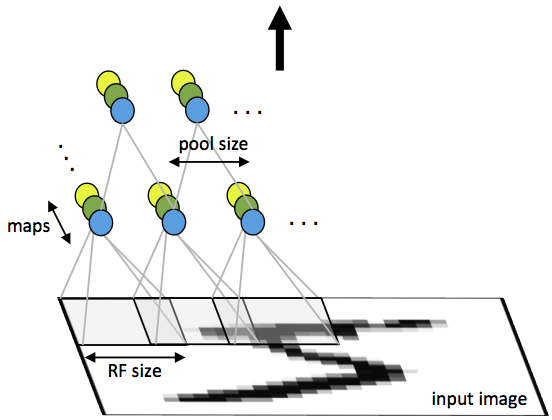
\includegraphics[scale=0.4]{Pictures/cnn.png}
		\rule{35em}{0.5pt}
		\caption[Convolutional Neural Network]{Convolutional Neural Network.}
		\label{fig:rnn}
\end{figure}

Further subsections discuss the considerations that go into designing these convolutional networks structures as well as optimisation and trainability conditions.
\subsection*{Filters}
The area covered by a filter (measured in pixel units) is called the \textit{receptive field size}. THe input image can be viewed as a volume of image size times the individual RGB values. So for an image of width $w$ and height $h$. The input volume would be $w*h*d$, where $d=3$ corresponding to each channel RGB. After applying $n$ filters of size $k*k$ each, we generate a layer of feature values of size $(w-k+1)*(h-k+1)*n$. Some methods of \textit{data augmentation} include adding of padded zeroes around the image that allow the filter to be applied in a manner that produce the same width and height dimensions for the output as the given input. This is useful for segmentation tasks discussed in the later sections.

The variable in this method of application of convolutions has three main variables.
\begin{itemize} \itemsep -2pt
\item \textit{Number of layers:} We can apply several layers of convolutional to generate intermediate representations of greater complexity. However greater complexity does not translate to better quality.  We can notice from the structure of the convolutional layers that the output of filters closer to the image data have a small receptive field, as the depth of the network increase, the output of every neuron is a function of a much larger area of the input image.
\item \textit{Dimension of filters:} The value of $k$ can be changed to modify the receptive field of each filter applied on the output of previous layers. While intuitively it might seem like a better idea to increase the receptive field size. It is shown experimentally that a larger filter dimension inhibits performance of the network. The added incentive of using smaller filter dimensions is the computational consideration. Due to the ability to parallelize the networks (discussed in sec.\ref{sec:impl}), smaller filters require lesser computation.
\item \textit{Number of filters per layer:} Every new feature map volume has a depth corresponding to the number of filters in the previous convolutional layer. Each filter is expected to behave as a unique feature detector from the repesentation space of the previous layer. The number of filters in each layer is an approximation of the number of features we expect to see in that layer. The output of a particular filter neuron is considered active if that feature is detected in the sub-volume equal to the receptive field size of that filter. Large number of filters cause the intermediate representation volumes to become very large. A pooling operation reduces the dimensionality of these volumes. It is essential to use a pool operation regardless of the input volume size for reasons discussed in the next section.
\end{itemize}

\subsection*{Pool}

As discussed in the earlier section, Every layer of applying convolutional filters creates a new \textit{volume}. Over subsequent layers these volumes can tend to become very large and store redundant data representations. Both issues are tackled by occasionaly including a \textit{pool} layer in between concolutional layers. A pool operation is applied to specific non-overlapping sub-volumes to produce a single output. This reduces the dimensionality of the input volume to each layer. Pooling also helps to make the representation become relatively invariant to small translations of the input. Invariance to translation implies that spatial displacement of lower level features will not affect the feature map of higher levels. This is desirable if the task to be performed is dependant on the existance of features rather than the location of the said features.

Some of the pool operations that are used are, \textit{max-pool}, \textit{avg-pool}, \textit{$L^2$ norm} from central pixel and several others. Empirically however, it has been seen that max-pool offers the best and most consistent performance. Moreover, operations such a max pool are easy to backpropagate through due their features discussed in Ch.\ref{ch:math}


\subsection*{Applications}
Various combinations of the above described elements give rise to a variety of possible network architectures with that can be used to solve different tasks.

\subsubsection*{Fully Convolutional Networks (FCNs)}
\subsubsection*{Regression}

\section{Recurrent Neural Networks (RNNs)}
Recureent Neural Networks, as the name suggests are networks with recurrent connections. A recurrent connvection induces the element of sequentiality to the network. We had earlier defined a Neural Network to be represented as a DAG. The introduction of a recurrent connection violates this definition due to the creation of a loop. This is reconciled (theoretically and computationally) by \textit{unfolding} the computational graph used for computing the values in the vanilla feedforward networks and the convolutional networks. The process of unfolding can be seen in fig.\ref{fig:rnn}

The rationale of an RNN is that the machine predicting the next element of a sequence of the value of the next time index is a function of the machine's state. A very rudimentary casting of this concept gives the following equation of a dynamic system,
\begin{equation}
\bm{s}^{(t)} = f(\bm{s}^{(t-1)};\bm{\theta})
\end{equation}
In the context of networks, using labeled training data, this equation takes the form,
\begin{equation}
\bm{h}^{(t)} = f(\bm{h}^{(t-1)},\bm{x}^{(t)};\bm{\theta})
\end{equation}
where $\bm{h}^{(t)}$ represents the state and $\bm{x}^{(t)}$ at time $t$.

\begin{figure}[H]
		\centering
		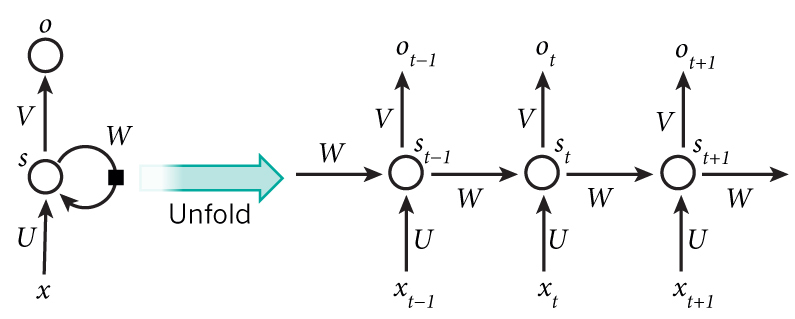
\includegraphics[scale=0.4]{Pictures/rnn.jpg}
		\rule{35em}{0.5pt}
		\caption[Recurrent Neural Network]{Recurrent Neural Network. \\ The left-hand side of the figure shows the unfolded version of a simplistic RNN, the black box on the self edge on the state node shows the addition of a time delay, thereby allowing the unfolding based on the time index of each input/ouput pair in the sequence.}
		\label{fig:rnn}
\end{figure}

The equations that correspond to the unfolded computational graph in fig.\ref{fig:rnn} can be stated as follows:
\begin{align*}
\bm{a}^{(t)} &= \bm b + \bm{Wh}^{(t-1)} + \bm{Ux}^{(t)} \\
\bm{h}^{(t)} &= tanh(\bm{a}^{(t)}) \\
\bm{o}^{(t)} &= \bm c + \bm{Wh}^{(t)}
\end{align*}

While training, the error is calculated via a loss function (usually \textit{cross-entropy loss}) by the following equation,
\begin{equation}
\hat{\bm y}^{(t)} = softmax(\bm{o}^{(t)})
\end{equation}
\subsection*{Training in RNNs}
Traditional backpropagation is evidently not possible for computing the gradients in an unfolded, due to the setup of the network. A modified version of the algorithm is required. It is called \textit{back-propagation over time} (BPTT) algorithm. THe calculation of the gradient starts at the last time step $\tau$ and propagates backward for each time step $t$. The original gradient will be,
\begin{align*}
\frac{\partial L}{\partial L^{(t)}} &= 1 \\
\left(\nabla_{\bm{o}^{(t)}}L\right)_{i} &= \hat{\bm{y}}_{i}^{(t)} - \bm 1 _{i,y^{(t)}} \\
\nabla_{\bm{h}^{(t)}}L &= \left(\frac{\partial \bm{h}^{(t+1)}}{\partial \bm{h}^{(t)}} \right) ^{\top}(\nabla_{\bm{h}^{(t+1)}}L) + \left(\frac{\partial \bm{o}^{(t)}}{\partial \bm{h}^{(t)}} \right) ^{\top} (\nabla_{\bm{o}^{(t)}}L)
\end{align*}
\section{High-Dimension Statistics}
\label{sec:highds}
In this section we address some the observations on the behaviour of multiple instances of networks and draw some statistical understanding on the reasons behind these behaviours. We use this information to analyse how these properties can be advantageous (or not) and how desirable properties can be created in networks.



